\chapter{\label{chap:lit-review}Revisão Bibliográfica}

\section{Spelunky}
Spelunky \cite{SPELUNKYWEB} é um jogo onde o jogador incorpora um aventureiro
que decide explorar uma caverna misteriosa. O local contém tesouros fabulosos,
mas também está repleto de perigos. O objetivo principal do jogador é explorar
estas cavernas subterrâneas e coletar a maior quantia de tesouros possível
enquanto evita ser abatido pelos diversos inimigos e armadilhas espalhadas pelo
ambiente. O jogo 2D segue o estilo \textit{platformer} - estilo de jogo
que envolve guiar um personagem através de plataformas suspensas e obstáculos
para obter progresso no jogo.

O jogo faz uso de alguns dos elementos-chave do gênero \textit{roguelike}, como
\textbf{geração procedural} e \textbf{morte permanente}. Os níveis em Spelunky
são gerados proceduralmente - ou seja, utiliza um algoritmo capaz de gerar
automáticamente os elementos que irão compor o nível - fazendo com que cada
partida seja única. Isto significa que não existe uma maneira de se ``decorar''
Spelunky, pois ao início de cada partida o mapa é gerado de maneira única e os
tesouros, itens e obstáculos são dispostos de maneira diferente, fazendo com que
o jogador tenha que aprender a lidar com os elementos de forma individual,
combinar este conhecimento e estabelecer uma estratégia para vencer seus
obstáculos e ser bem sucedido. Além disso, o jogo conta com o conceito de morte
permanente, que faz com que o jogador, ao ter o seu número de vidas esgotado,
tenha que recomeçar o jogo desde o seu início, perdendo todo o progresso obtido
até então.

O jogo é dividido em 4 áreas principais: \textbf{As Minas}, \textbf{A Selva},
\textbf{As Cavernas De Gelo} e \textbf{O Templo}. Cada área possúi um estilo de
mapa e aparência única. O nível de dificuldade também aumenta gradativamente,
principalmente porque os inimigos vão se tornando cada vez mais fortes. Além das
áreas principais, existem duas áreas secretas: \textbf{O Mercado Negro} e
\textbf{A Cidade de Ouro}.

O jogador, inicialmente, conta somente com um chicote, 4 pontos de vida, 4
bombas e 4 cordas para ajudá-lo a se defender e se locomover pela caverna.
Contudo, diversos equipamentos, acessórios e armas podem ser obtidos e
utilizados ao longo do jogo. Além disso, o jogador pode interagir com objetos do
ambiente, como pedras, vasos, baús de tesouro, entre outros. Também se
encontram, espalhados pelas cavernas, os \textbf{Comerciantes}. Estes
\textit{NPCs}\footnote{\textit{Non-Playable Characters}(Personagens
Não-Jogáveis). São personagens que não são controlados pelo jogador. Geralmente
interagem de alguma maneira com o personagem do jogador.} comercializam itens
com o jogador em troca de tesouros. É possível, inclusive, tentar furtar itens
destes comerciantes. Contudo, se o jogador o fizer, todos os comerciantes
ficarão extremamente irritados e passarão a caçar o explorador com espingardas.

O jogo foi desenvolvido por Derek Yu - utilizando o motor de desenvolvimento de
jogos \textit{GameMaker} (Versão 8) - e lançado gratuitamente para a plataforma
\textit{Windows} em dezembro de 2008\cite{SPELUNKYRELEASE}. No fim de 2009, o
criador optou por liberar o código fonte do jogo, permitindo sua distribuição
não-comercial e modificação\cite{SPELUNKYLICENSE}.

O uso do motor GameMaker para o desenvolvimento do jogo faz com que seja
possível o uso de ferramentas que facilitam o trabalho do desenvolvedor.
Contando com funcionalidades como editores de \textit{scripts}\footnote{Código
desenvolvido para o controle dos comportamentos dos elementos do jogo.} e de
\textit{sprites}\footnote{Elementos visuais do jogo, tais como o personagem, o
fundo, os inimigos. Representados como uma ou mais imagens, permitindo que as
mesmas sejam animadas.}, gerenciadores de eventos, entre outras
\cite{GMAKER8DOCS}, o GameMaker oferece um ótimo suporte ao desenvolvedor para a
criação de jogos.

\begin{figure}[htb!]
\centering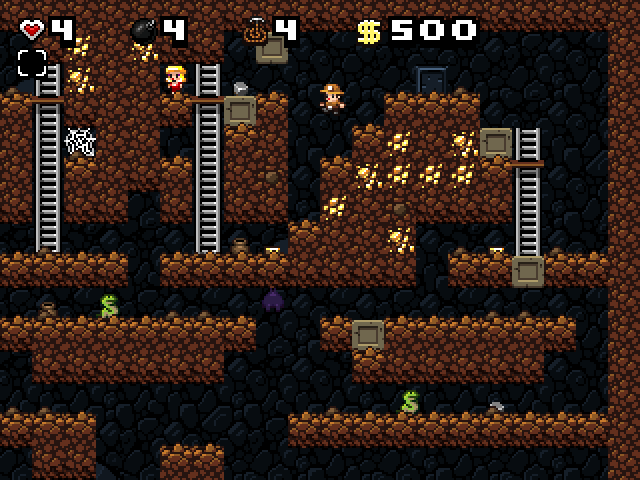
\includegraphics[width=.65\textwidth]{fig/spelunky-pc-screen.png}
\caption {\label{fig:spelunky-gameplay}Exemplo de partida de spelunky, mostrando
elementos do jogo como o jogador, a caverna, os inimigos, os tesouros, entre
outros.} \end{figure}



\section{Plataformas de Testes para Inteligência Artificial}
Existe uma relação mutualmente benéfica entre a área de inteligência artificial
e jogos digitais.  De um lado, os jogos se beneficiam explorando conceitos,
técnicas e algoritmos de inteligência artificial com o intuito de enriquecer
seu conteúdo. O jogo \textbf{Black \& White} da desenvolvedora \textit{Lionhead
Studios}, por exemplo, incorporou as técnicas de agentes BDI, árvores de
decisão e redes neurais para ditar o comportamento de alguns seus personagens
\cite{TOPAIGAMES}. Já o jogo \textbf{F.E.A.R}, da desenvolvedora
\textit{Monolith Productions}, utilizou os conceitos de planejamento para
aumentar o realismo das decisões tomadas por seus agentes.\cite{FEARPLANNING}.

Do outro lado, o campo da inteligência artificial se beneficia ao utilizar os
jogos como plataformas de teste para suas técnicas e algoritmos. Jogos digitais
são capazes de capturar a complexidade de situações do mundo real e, ao mesmo
tempo, manterem-se relativamente simples e baratos. Podem replicar inúmeras
situações e ambientes -- existem diversos gêneros de jogos, variando desde
jogos educacionais até jogos de tiro em primeira pessoa -- e até mesmo criar
cenários impossíveis ou impraticáveis no mundo real. Ademais, possuem a
vantagem de serem programas de computador, o que significa que, por muitas
vezes, podem acelerar a velocidade na qual testes são executados, ou ainda
executar múltiplos testes em paralelo. A natureza lúdica dos jogos também são
um ponto importante a ser ressaltado, pois ajudam a motivar os pesquisadores,
além de resultar na adesão de outros. Estas são algumas das características dos
jogos digitais que fazem com que sejam atraentes para pesquisadores da área de
inteligência artificial.

Tendo este apanhado de informações em mente, pesquisadores e entusiastas da
área acabam desenvolvendo \textit{frameworks} de inteligência artificial em
cima de jogos existentes para servir de plataforma de teste. Um exemplo disso
seria o \textbf{Brood War API} \cite{BWAPI}, um \textit{framework} para o jogo
\textit{StarCraft: Brood War}. Algumas vezes, contudo, são criados jogos
especificamente para isso, como foi o caso do projeto \textbf{TORCS, The Open
Racing Car Simulator}, um simulador de corridas de carro que permite que
desenvolvedores programem a inteligência de carros e compitam entre sí
\cite{TORCSWEB}.

\subsection{Competições de Inteligência Artificial em Jogos Digitais}
Muitas vezes, os \textit{frameworks} de inteligência artificial desenvolvidos
dão origem a competições, servindo como base comum para o desenvolvimento e
aplicação de técnicas de inteligência artificial para os concorrentes. Nestas
disputas, os competidores são encorajados a resolver problemas ou sub-problemas
impostos pelo jogo em questão, sendo vencedores os candidatos que melhor
resolvê-los.

Geralmente, o problema proposto é o de jogar o jogo de maneira mais eficiente.
Para realizar uma avalição objetiva, são utilizadas métricas estipuladas pelo
próprio jogo, como pontuação ou tempo. Muitas vezes, os organizadores da
competição optam por fazer uso de um sistema de \textit{ranking}, expondo os
resultados obtidos pelos candidatos. A competição \textbf{The General Video
Game AI Competition}, que explora o problema de criar controladores genéricos
de jogos, faz uso deste mecanismo \cite{GVGAIWEB}.  Frequentemente, também,
fazem com que os candidatos joguem entre sí.  Um exemplo disso seria a
competição que gira em torno de \textbf{Vindinium}, um jogo para a plataforma
\textit{web} \cite{VINDINIUMWEB}.

Contudo, a proposta principal da disputa pode ser outra. A competição
\textbf{Mario AI Competition}, por exemplo, possuia como uma de suas metas a
criação de níveis interessantes para o jogo \cite{MARIOAIWEB}. Já a competição
\textbf{2K Bot Prize} tinha como objetivo a criação de uma inteligência
artificial para o jogo \textit{Unreal Tournament 2004} que pudesse enganar
outros jogadores e fazê-los pensar que era um humano jogando.
\cite{UNREALAIWEB}. Neste tipo de torneio, a avaliação se dá de maneira
subjetiva, visto que não existe uma métrica numérica para determinar diversão,
por exemplo.

Os organizadores destas competições costumam, ao término da disputa,
disponibilizar os códigos-fonte de todos os candidatos. Assim, em versões
futuras da competição, os competidores terão a oportunidade de investigar quais
técnicas e algoritmos foram mais eficientes no passado. Em competições onde os
candidatos duelam entre sí, isto tende a aumentar a competitividade, pois uma
solução que funcionou em um ano pode vir a não funcionar tão bem ou até mesmo
falhar no ano seguinte, tendo em vista que o código será dissecado pelos seus
rivais. Os resultados das competições costumam ser divulgados também em
conferências como \textit{IEE Computational Intelligence and Games (CIG)} e
\textit{AAAI Artificial Intelligence in Interactive Digital Entertainment
(AAIDE)}, além de conferências dedicadas a computação evolutiva, \textit{game
design}, aprendizado de máquina, entre outras. Algumas competições costumam
oferecer prêmios em dinheiro para os melhores colocados, como forma de
incentivo.



\section{SpelunkBots}
Falar em especifico sobre o SpelunkBots



\section{Agentes Racionais}
Um agente pode ser visto como todo e qualquer tipo de entidade que seja capaz de
perceber o ambiente onde está situado, através de seus sensores, podendo
executar ações nesse ambiente conforme sua necessidade através de seus
atuadores.\cite{Russell:1995:AIM:193191}

Para exemplificar, podemos tomar como exemplo o ser humano, que consegue
perceber o ambiente através de seus olhos e ouvidos, por exemplo, conseguindo
agir no ambiente com suas partes do corpo, como braços, pernas, mãos e etc.
\cite{Russell:1995:AIM:193191}

Portanto, podemos generalizar o conceito de agente racional como todo e qualquer
tipo de agente que, no ambiente em que está inserido, toma ações que o deixam
mais próximo de completar os objetivos os quais o mesmo está comprometido.

\subsection{Agentes Reflexivos}
Agentes reflexivos são agentes que executam ações baseados em alguma situação
percebida. Por exemplo, podemos ter um agente reflexivo que poderá fazer uma
postagem em uma rede social, dado que uma outra pessoa fez uma postagem. Tal
tipo de agente não ``pensará'' sobre a ação que está executando, simplesmente a
executará baseado no que percebeu anteriormente.

Estes agentes têm como principal característica não guardarem tipo algum de
informação das suas experiências passadas, sendo apenas reativos.

\subsection{Agentes com Memória}
Diferentemente dos agentes reflexivos, agentes com memória são capazes de
guardar informações sobre as experiências passadas, podendo fazer o uso das
mesmas para alcançar seus objetivos. A lembrança das experiência passadas
possibilita à um agente uma forma de aprender e melhorar, fazendo com que, por
exemplo, sejam evitadas ações não efetivas ou que seja escolhida, entre um
conjunto de possíveis ações, a que seja a mais efetiva para o agente.

\subsection{Agentes Baseados em Objetivos}
Além de ter memória, é necessário que um agente saiba quando o mesmo obteve
sucesso no que se propôs a fazer. Com isso, agentes baseados em objetivos
conseguem basear suas decisões - ações a tomar - com base na ação que o deixa
mais próximo de alcançar seus objetivos. O desafio desse tipo de agente é saber
como alcançar esse objetivo, podendo ser usadas técnicas de busca e planejamento
para determinar as possíveis ações a serem executadas para alcançá-lo.

\subsection{Agentes Baseados em Utilidades}
Para alguns tipos de agente, chegar no objetivo pode não ser suficiente, podendo
existir outros fatores na busca desse objetivo que possam influenciar no
resultado final do agente. Por exemplo, um agente que joga um determinado jogo
pode terminar o jogo com um determinado número de pontos, porém, é mais
satisfatório que o mesmo termine o jogo com o \textbf{maior} número de pontos
possível.

Portanto, tais tipos de agentes são capazes de medir os resultados de suas
ações, escolhendo as que, além de alcançar seu objetivo, façam o mesmo da melhor
maneira possível.

\subsection{Ambiente}
Todas as ações que um agente pode executar, bem como suas percepções, ocorrem no
ambiente onde o agente está inserido. Porém, existem diferentes tipos de
ambientes, que, dependendo de sua característica, podem dificultar o trabalho de
um determinado agente.

Primeiramente, os ambientes podem ser \textbf{acessíveis} ou
\textbf{inacessíveis} (também chamados de \textbf{observáveis} ou \textbf{não
observáveis}), sendo um ambiente acessível aquele que possibilita que o agente
explore todas as suas características. Ambientes acessíveis permitem que o
agente não precise guardar informações sobre o mesmo, visto que pode sempre
``olhar'' para o ambiente e extraír as informações necessárias.

Também existem os ambientes \textbf{determinísticos} ou \textbf{estocásticos},
tratando-se de um ambiente deterministico aquele onde um agente consegue prever
o próximo estado da sua busca pelo objetivo através da aplicação das ações
escolhidas. Assim, um ambiente não determinístico não garante que a ação
executada pelo agente irá surtir o efeito esperado.

Além destes, existem ambientes \textbf{episódicos} ou \textbf{sequenciais},
sendo ambientes episódicos aqueles onde um episódio não influencia no próximo.
Dessa forma, ambientes sequenciais guardam algum tipo de memória dos epoisódios
anteriories, fazendo o uso desta nos episódios subsequentes, gravando outras
informações sobre tais episódios caso necessário.

Caso um ambiente possa sofrer mudanças sem ações do agente, será um ambiente
\textbf{dinâmico}, caso contrário, chamamos esse tipo de ambiente de
\textbf{estático}. Caso o ambiente não mude de acordo com o tempo, porém, o
agente mude sua forma de agir (melhorando sua atuação, por exemplo), chamamos
o ambiente de \textbf{semidinâmico}.

Por fim, classificamos os ambientes como \textbf{discretos} ou
\textbf{contínuos}, sendo ambientes discretos aqueles onde temos um número
finito de possíveis estados.

Dados os seguintes tipos:

\begin{enumerate}
    \item Acessível
    \item Determinístico
    \item Episódico
    \item Estático
    \item Discreto
\end{enumerate}

Podemos exemplificar os tipos de ambientes através da
tabela~\ref{tab:ENVEXAMPLETABLE}:

\begin{table}[htb]
    \begin{center}
        \caption{\label{tab:ENVEXAMPLETABLE} Tabela exemplificando os
        diferentes tipos de ambientes}
        \begin{tabular}{| l | c | c | c | c | c |} \hline
            \textbf{Tipo de Ambiente}         & \textbf{1} & \textbf{2} & \textbf{3} & \textbf{4} & \textbf{5} \\ \hline
            Partida de xadrez sem relógio     & Sim        & Sim        & Não        & Não        & Não        \\ \hline
            Corrida de táxi                   & Não        & Não        & Não        & Não        & Não        \\ \hline
            Partida de poker                  & Não        & Não        & Não        & Sim        & Sim        \\ \hline
            Sistema para diagnósticos médicos & Não        & Não        & Não        & Não        & Não        \\ \hline
            Sistema para análise de imagens   & Sim        & Sim        & Sim        & Semi       & Não        \\ \hline
        \end{tabular}
    \end{center}
\end{table}

\subsection{Agentes BDI}
O estudo de agentes racionais faz com que seja necessário, além de entender os
aspectos e característica dos mesmos, entender como é possível realizar a
implementação desse tipo de agente.

A aplicação de técnicas convencionais para o desenvolvimento desses agentes
mostrou-se despendiosa e difícil de ser feita, verificada e mantida
\cite{BDIFROMTHEORYTOPRACTICE}, sendo então necessária o uso de outras técnicas
para a implementação dos mesmos.

Nesse contexto, surge a arquitetura de agentes BDI (\textit{Belief, Desire,
Intentions}), capaz de modelar agentes racionais de uma maneira mais adequada.

Tal arquitetura conta com alguns conceitos que permitem modelar agentes
racionais, explicados a seguire:

\begin{description}
    \item [Crenças (\textit{Beliefs})]
        Trata-se de tudo aquilo que o agente acredita saber sobre o ambiente,
        é chamado de ``crença'' pois tal informação pode vir a não ser verdade.
        As crenças podem vir a ser atualizadas a cada nova percepção do ambiente
        feita pelo agente, sendo armazenadas na memória do agente.
    \item [Desejos (\textit{Desires})]
        Além de uma base de crenças, é necessário que um agente saiba o que deve
        ser feito para alcançar os seus objetivos. Tais ações são chamadas de
        desejos, e, além de representar o que um agente deseja fazer, também
        representam os custos associados com a busca por esse desejo.
    \item [Intenções (\textit{Intentions})]
        Diferentemente dos desejos, uma intenção é algo com o qual o agente se
        compromete a fazer em busca dos seus objetivos, dessa forma, podemos ver
        as intenções como as ações que efetivamente serão executadas para
        alcançar os objetivos.
\end{description}

Com estes três conceitos, é possível definir um algoritmo interpretador
BDI. O algoritmo~\ref{alg:BDIINTERPRETERALG} mostra como é feito o uso desses
conceitos \cite{BDIFROMTHEORYTOPRACTICE}.

\begin{algorithm}[htb]
\begin{center}
    % Um exemplo de algoritmo utilizando a pacote 'algorithmic'
    %\algsetup{linenosize=\small,linenodelimiter=.}
    \begin{algorithmic}[1]
        \STATE inicializar();
        \STATE
        \WHILE {true}
            \STATE opções $\gets$ gerar-opções(fila-de-eventos);
            \STATE opções-escolhidas $\gets$ deliberar(opções);
            \STATE atualizar-intenções(opções-escolhidas);
            \STATE executar();
            \STATE buscar-novos-eventos-externos();
            \STATE esquecer-atitutes-de-sucesso();
            \STATE esquecer-atitudes-impossíveis();
        \ENDWHILE
    \end{algorithmic}
\end{center}
\caption[Algoritmo para representar um interpretador BDI.]
    {\label{alg:BDIINTERPRETERALG}
        Algoritmo para representar um interpretador BDI, utilizando os conceitos
        de crenças, desejos e intenções para a sua implementação.}
\end{algorithm}

As possíveis opções são escolhidas a cada novo ciclo, sendo sempre buscadas de
uma fila de eventos ocorridos, após, é escolhida uma opção a ser seguida,
tornando-se então essa opção uma intenção do agente. Caso haja uma intenção a
ser executada, o agente então a executa. Após, é atualizada a fila de eventos
com os eventos externos ocorridos. Por fim, o agente esquece os desejos já
obtidos, bem como as intenções satisfeitas, além de esquecer os desejos e
intenções impossíveis.

Por fim, cabe ressaltar que tal arquitetura possui algumas limitações, bem como
a incapacidade de fazer com que um agente BDI ``aprenda'' e adapte seu
comportamento baseado no aprendizado obtido, além de não haver nenhuma
consideração arquitetural sobre a modelagem de sistemas multi-agentes
\cite{BDIMODELOFAGENCY}, sendo assim necessário explorar outras técnicas caso
seja necessário que o agente faça uso dessas características.

\section{Planejamento}

A solução para muitos tipos de problemas pode ser expressa através de uma
sequência de ações a serem executadas - isto é, um plano - principalmente quando
temos algum tipo de restrição no ambiente. Portanto, em muitos casos, é
necessário que um agente estabeleça um plano sobre o que deve ser feito para
resolver o problema o qual foi designado, seguindo as ações que resolvam o
mesmo.

Tomemos como exemplo um agente em um ambiente estocástico - onde não se consegue
ter certeza sobre o resultado da execução de uma ação - e não observável, como
não temos certeza sobre o estado do ambiente, nem sobre o resultado de nossas
ações, precisamos estabelecer um plano onde podemos tratar as dificuldades que
o ambiente nos impõe.

Portanto, podemos definir um sistema planejador como um sistema que tem como
saída um plano a ser executado e como entrada os seguintes componentes:

\begin{description}
    \item [Objetivos]
        Também chamados de intenções ou tarefas, é algo que o agente deseja
        obter, manter ou evitar.
    \item [Crenças]
        Tudo o que um agente sabe sobre o estado do ambiente.
    \item [Ações]
        Tudo o que um agente pode executar no ambiente onde está inserido.
\end{description}\cite{Woolridge:2001:IMS:559667}

A ideia principal para a construção de um sistema planejador se dá através da
extensão da representação de crenças, objetivos e ações com o uso de algum tipo
de linguagem formal (normalmente lógica de primeira ordem, ou algum subconjunto
da mesma). Isso permite que o planejador possa fazer uma ligação direta entre
as ações e os estados, podendo, portanto, considerar apenas ações relevantes
para o plano.
\cite{Russell:1995:AIM:193191}

As ações passam a ter pré-condições e efeitos, que faz com que o agente, antes
de executar uma ação, tenha que ter um conhecimento prévio do ambiente. Assim,
após a execução da mesma, seus efeitos fazem com que seja alterado o
conhecimento sobre o ambiente.

O uso de uma linguagem formal nessa tarefa permite que os componentes de um
planejador sejam expressos de uma maneira onde seja possível fazer operarações
sobre tais conjecturas, facilitando o processo de geração de um plano.

Um dos primeiros planejadores a surgir foi o STRIPS \cite{STRIPSNEWAPPROACH},
em $1971,$ sendo utilizado como referência para a solução de muitos problemas de
planejamento até hoje.

\section{Aprendizado de Máquina}

\begin{itemize} \item O que é \item Para que serve \item Como se faz (forma
abstrata) \end{itemize}

\subsection{Aprendizado por Reforço}

Explicar de uma forma genérica, talvez citar as áreas relacionadas

\subsection{Q-Learning}

Explicar o algoritmo

\subsection{SARSA}

Explicar o algoritmo

\subsection{Deep Learning}

TBD
